%!TEX root = ../BUSystematics.tex

\graphicspath{{Body/Figures/Gain/IFG/60h/Amplitude/}{Body/Figures/Gain/IFG/60h/Amplitude-With-AdHoc/}{Body/Figures/Gain/IFG/60h/Lifetime/}{Body/Figures/Gain/IFG/9d/Lifetime/}{Body/Figures/Gain/ResidualGain/EnergyBinKloss/}{Body/Figures/Gain/ResidualGain/Chi2Min/}}

\section{Gain Systematic Uncertainties}


Detected positon energies are corrected for in-fill, short-term, and out-of-fill gain corrections (IFG, STDP, OOF) \cite[and references therein]{GainNote}. A laser system was used to determine these corrections and the parameters associated with them. Uncertainties in the IFG and STDP correction parameters propagate into uncertainties on the extracted \wa values\footnote{The OOF correction acts on time scales much larger than a fill, and so does not add a systematic uncertainty.}. Lastly and separately, a systematic uncertainty was evaluated in regards to the possible need for a residual or ad-hoc gain correction.



\subsection{IFG Amplitude and Time Constant}


The IFG correction is given by
\begin{align}
  E_{t} = E_{m}/(1 - A_{IFG} e^{-t/\tau_{IFG}}),
\end{align}
where $E_{t}$ is the true energy of the detected positron, $E_{m}$ is it's measured energy, and $A_{IFG}$ and $\tau_{IFG}$ are the amplitude and time constant parameters used in the correction. The systematic uncertainties on \wa (or \R\footnote{\R is related to \wa via the equation
\begin{align}
  \omega_{a} = 2\pi \cdot \SI{0.2291}{MHz} \cdot (1 + (R - \Delta R) \times 10^{-6}),
\label{eq:wa}
\end{align}
where $\Delta R$ is a blinding offset.}) due to the uncertainties in the amplitude and time constant parameters were evaluated by scanning over those parameters in multiplicative steps, determining the sensitivity of \R to those parameters, and multiplying by the respective parameter errors:
    \begin{align}
        \delta R = \sigma_{(A_{IFG}, \tau_{IFG})} \times \frac{dR}{d(A_{IFG}, \tau_{IFG})}.
    \end{align}


The uncertainties in the IFG (and STDP) parameters are given in \tabref{tab:gainCorrErrs}. These uncertainties were evaluated by D. Sweigart, where he calculated the average crystal parameter uncertainties weighted by the counts put into his T-Method histogram. Note that the IFG parameter uncertainties for the HighKick and Endgame datasets are noticeably less than those of the 60h and 9d datasets. This is because the time constants in the IFG corrections were set to those values determined from long-term double pulse studies (LTDP) \cite{GainNote}, rather than IFG correction studies\footnote{Connected to this fact is that for the 60h and 9d datasets, the gain corrections were applied in the order \{OOF, STDP, IFG\}, whereas for the HighKick and Endgame datasets, the order was \{STDP, OOF, IFG\}.}. This resulted in more accurately determined values and therefore smaller parameter uncertainties.


\begin{table}
\centering
\setlength\tabcolsep{10pt}
\renewcommand{\arraystretch}{1.2}
\begin{tabular*}{1\linewidth}{@{\extracolsep{\fill}}lHHHH}
  \hline
    \multicolumn{5}{c}{\textbf{Gain Correction Parameter Uncertainties}} \\
  \hline
    Quantity & \thead{60h} & \thead{HighKick} & \thead{9d} & \thead{Endgame} \\
  \hline
    IFG Amplitude      & 21.4 & 6.3 & 15.3  & 3.7 \\
    IFG Time Constant  & 16.1 & 6.5 & 11.5 & 6.5 \\
    STDP Amplitude     & 1.9 & 1.9 & 1.9 & 1.9 \\
    STDP Time Constant & 3.4  & 3.4 & 3.4 & 3.4 \\
  \hline 
\end{tabular*}
\caption[]{Average uncertainties on the crystal gain correction parameters, in percent, weighted by the number of counts put into the T-Method histogram, as determined by D. Sweigart. For sources on the numbers see the left side of Table~6.5 in \refref{phdthesis:2020Sweigart} for the 60h and 9d datasets, and the Run~1 uncertainty spreadsheet for the HK and EG datasets \cite{UncertaintySpreadsheet}. Original gain correction data can be found in \cite{GainElog1,GainElog2,GainElog3,GainElog4}. All STDP parameters were the same as they were calculated from the same laser data. The author calculated the average (not hit-weighted) uncertainties, and found less than a percent difference in each case.}
\label{tab:gainCorrErrs}
\end{table}




\figref{fig:IFGAmpscan} shows the fitted \R and \chisq values for the T- and R-Methods versus the multiplier on the IFG amplitude for the 60h dataset. The sensitivity was determined by fitting a straight line to the \R versus amplitude multiplier plot in the range 0--2. These sensitivities in general are minimized when the fit start time is chosen such that it lies on \gmtwo zero crossing. Similarly, Figures~\ref{fig:IFGtauscan} and \ref{fig:IFGtauscan9d} show the fitted \R and \chisq values versus the multiplier on the IFG time constant for the 60h and 9d datasets respectively. Whereas the trends for \R versus the amplitude are linear, the shape is a little more complex for the time constant. For the 60h and HighKick datasets the shape starts off flat at a multiplier of 0, dips down a bit as it approaches a multiplier of 1, and then rises linearly. For the 9d and Endgame datasets, the trend is the same, except that at higher multipliers around 1.5, the trend starts to drop. This difference in behavior versus the lifetime is connected to the fact that the LTDP time constants were used for the 9d and Endgame datasets. In order to evaluate the errors consistently among the different datasets, the sensitivities were extracted by fitting a straight line to the plots with the same range. That range was determined via inspection of the various plots, and set to 0.8--1.5, such that the linear region was used in all datasets. 



\begin{figure}[h]
\centering
    \begin{subfigure}[t]{0.45\textwidth}
        \centering
        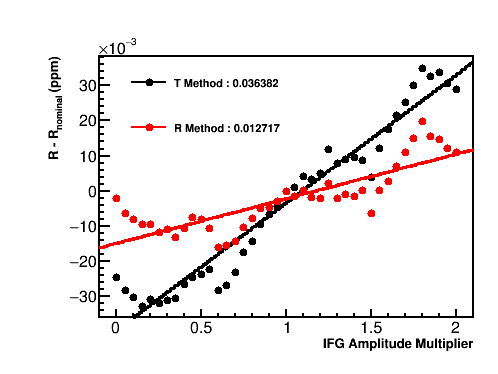
\includegraphics[width=\textwidth]{IFG_Amplitude_Compare_R}
        % \caption{}
    \end{subfigure}% %you need this % here to add spacing between subfigures
    \hspace{1cm}
    \begin{subfigure}[t]{0.45\textwidth}
        \centering
        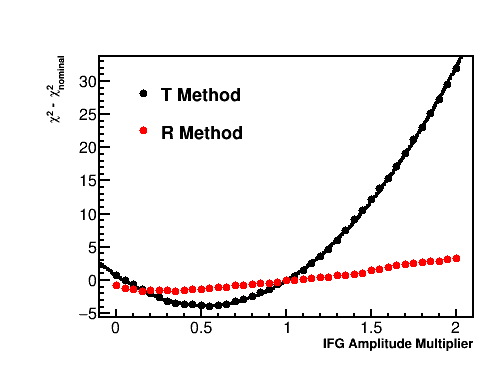
\includegraphics[width=\textwidth]{IFG_Amplitude_Compare_Chisq}
        % \caption{}
    \end{subfigure}
\caption[]{\R (left) and \chisq (right) versus the multiplier on the IFG amplitude parameter, for the T- and R-Methods. The sensitivities of \R to the parameter is determined by fitting a line to the points in the range 0--2, and the extracted values are included in the plot in units of ppm per unit amplitude. It should be noted that the fluctuations in the points are statistical in nature. As shown the sensitivity of the R-Method to the IFG amplitude is less than that of the T-Method. For the \chisq plot, the T-Method forms a parabola and finds a minimum far from the nominal multiplier of 1, which is evidence for the need for a residual gain correction, \secref{sub:residual_gain_correction}. The R-Method with it's reduced sensitivity does not form a parabola. Data are from the 60h dataset.}
\label{fig:IFGAmpscan}
\end{figure}



\begin{figure}[h]
\centering
    \begin{subfigure}[t]{0.45\textwidth}
        \centering
        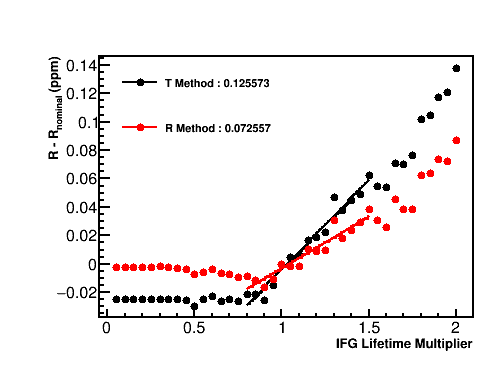
\includegraphics[width=\textwidth]{IFG_Lifetime_Compare_R}
        % \caption{}
    \end{subfigure}% %you need this % here to add spacing between subfigures
    \hspace{1cm}
    \begin{subfigure}[t]{0.45\textwidth}
        \centering
        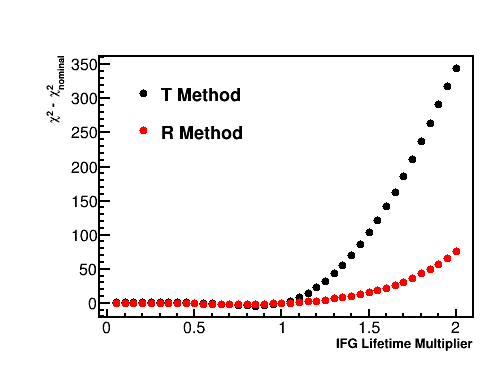
\includegraphics[width=\textwidth]{IFG_Lifetime_Compare_Chisq}
        % \caption{}
    \end{subfigure}
\caption[]{\R (left) and \chisq (right) versus the multiplier on the IFG time constant parameter, for the T- and R-Methods, for the 60h dataset. The sensitivities of \R to the parameter is determined by fitting a line to the points in the range 0.8--1.5, and the extracted values are included in the plot in units of ppm per unit time constant. As shown the sensitivity of the R-Method to the IFG amplitude is less than that of the T-Method.}
\label{fig:IFGtauscan}
\end{figure}


\begin{figure}[h]
\centering
    \begin{subfigure}[t]{0.45\textwidth}
        \centering
        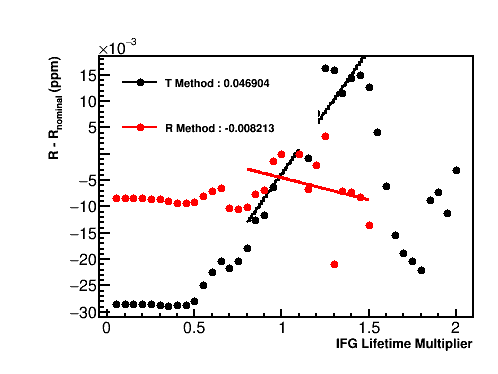
\includegraphics[width=\textwidth]{IFG_Lifetime_Compare_R_9d}
        % \caption{}
    \end{subfigure}% %you need this % here to add spacing between subfigures
    \hspace{1cm}
    \begin{subfigure}[t]{0.45\textwidth}
        \centering
        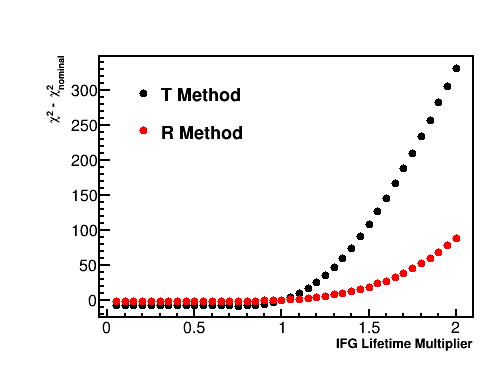
\includegraphics[width=\textwidth]{IFG_Lifetime_Compare_Chisq_9d}
        % \caption{}
    \end{subfigure}
\caption[]{\R (left) and \chisq (right) versus the multiplier on the IFG time constant parameter, for the T- and R-Methods, for the 9d dataset. The sensitivities of \R to the parameter is determined by fitting a line to the points in the range 0.8--1.5, and the extracted values are included in the plot in units of ppm per unit time constant. As shown the sensitivity of the R-Method to the IFG amplitude is less than that of the T-Method. \R versus the time constant for the 9d and Endgame datasets falls off at high multipliers, due to a different procedure for determining the time constants in the IFG correction in those two datasets.}
\label{fig:IFGtauscan9d}
\end{figure}





\tabref{tab:IFGResults} gives the sensitivities to the IFG amplitude and time constant parameters for the four Run~1 datasets, and the associated systematic errors after those sensitivities have been multiplied against the corresponding errors in \tabref{tab:gainCorrErrs}. As shown the errors are small, $\mathcal{O}(10)$ ppb. 




\begin{table}[h]
\centering
% \setlength\tabcolsep{10pt}
\renewcommand{\arraystretch}{1.2}
\begin{tabularx}{0.9\linewidth}{XcYKYK}
  \hline
    \multicolumn{6}{c}{\textbf{IFG Systematic Uncertainties}} \\
  \hline\hline
    Dataset & \thead{Fit Method} & \multicolumn{1}{c}{$dR/dA_{IFG}$} & \multicolumn{1}{c}{$\boldsymbol{\delta R_{A_{IFG}}}$} & \multicolumn{1}{c}{$dR/d\tau_{IFG}$} & \multicolumn{1}{c}{$\boldsymbol{\delta R_{\tau_{IFG}}}$} \\
  \hline
    \multirow{2}{*}{60h} & T & 36.4 & 7.8 & 125.6 & 20.2 \\
                         & R & 12.7 & 2.7 & 72.6 & 11.7 \\
  \hline
    \multirow{2}{*}{HighKick} & T & 52.1 & 3.3 & 150.4 & 9.8 \\
                              & R & 8.4 & 0.5 & 49.7 & 3.2 \\
  \hline
    \multirow{2}{*}{9d} & T & 29.6 & 4.5 & 46.9 & 5.4 \\
                        & R & 9.7 & 1.5 & 8.2 & 0.9 \\
  \hline
    \multirow{2}{*}{Endgame} & T & 64.0 & 2.4 & 204.5 & 13.3 \\
                             & R & 27.9 & 1.0 & 101.3 & 6.6 \\
  \hline
\end{tabularx}
\caption[]{Sensitivities of \R to IFG parameters for the four Run~1 datasets. Units are in ppb per unit amplitude, ppb per unit time constant, and ppb, for the sensitivities and systematic uncertainties respectively.}
\label{tab:IFGResults}
\end{table}





\clearpage
\subsection{STDP}


The systematic uncertainty due to the STDP correction was evaluated by turning the STDP correction entirely off before reclustering the hits. The changed in \R, \DR, was multiplied by the uncertainty in STDP amplitude as given in \tabref{tab:gainCorrErrs} to determine the uncertainty. The Run~1 analysis did not have the capability to scan over the STDP parameters as was done for the IFG, hence the single point chosen with an amplitude of 0\footnote{This is being fixed for future analyses.}. It should be noted that because of the nature of how the randomization is applied in the BU analysis, the change in \R was completely disassociated from any randomization effects, and is solely due to the change in gain. \tabref{tab:systematicError_STDP} gives the \DR's with the STDP turned off, along with the systematic uncertainties for the four datasets and both fit methods. As shown the systematic uncertainties are entirely negligible at less than 1~ppb. Because the systematic uncertainties were so small, a systematic uncertainty regarding the STDP lifetime was not evaluated.


\begin{table}[h]
\centering
% \setlength\tabcolsep{10pt}
\renewcommand{\arraystretch}{1.2}
\begin{tabularx}{0.7\linewidth}{XOOK}
  \hline
    \multicolumn{4}{c}{\textbf{STDP Systematic Uncertainties}} \\
  \hline\hline
    Dataset & \thead{Fit Method} & \multicolumn{1}{c}{$\Delta R_{\text{(w/ - w/o)}}$} & \multicolumn{1}{c}{$\boldsymbol{\delta R}$} \\
  \hline
    \multirow{2}{*}{60h} & T & 4.8 & 0.1 \\
                         & R & 2.8 & 0.1 \\
  \hline
    \multirow{2}{*}{HighKick} & T & 2.2 & 0.1 \\
                              & R & 2.2 & 0.1 \\
  \hline
    \multirow{2}{*}{9d} & T & 11.2 & 0.2 \\
                        & R & 14.0 & 0.3 \\
  \hline
    \multirow{2}{*}{Endgame} & T & 3.9 & 0.1 \\
                             & R & 5.0 & 0.1 \\
  \hline
\end{tabularx}
\caption[]{Changes in \R with versus without the STDP effect applied for both fit methods for all four datasets, along with the associated systematic uncertainties. These uncertainties were evalued by multiplying the \DR's by the error on the STDP amplitude as given in \tabref{tab:gainCorrErrs}. Units are in ppb.}
\label{tab:systematicError_STDP}
\end{table}








\subsection{Residual Gain Correction}
\label{sub:residual_gain_correction}


In Run~1 (and potentially for future runs) there were several pieces of evidence that pointed towards the need for a residual or ad-hoc gain correction. These included fit start time scans for the $N$, $\tau_{\mu}$, and \K parameters which fell outside the $1\sigma$ allowed difference bands, IFG amplitude scans which found minima far from the nominal multiplier of 1 (see \figref{fig:IFGAmpscan}), and the \K versus energy spectra which falls at high energies as opposed to remaining constant \cite{phdthesis:2019Fienberg,phdthesis:2020Sweigart,AdHoc1,AdHoc2}. A. Fienberg proposed an additional gain correction with the form
\begin{align}
  E_{c} = E_{m} \cdot (1 + A_{g} e^{-t/\tau_{\mu}} (1 + 0.2 \cos(\omega_{a}t + \phi))),
\end{align}
where $E_{c}$ is the corrected energy of the detected positron, $E_{m}$ is it's measured energy, and $A_{g}$ is the amplitude of the correction. The asymmetry value of 0.2 on the oscillatory part was determined as the ``overall asymmetry of the energy-weighted hit rate'' \cite{phdthesis:2019Fienberg}. \taumu was set to the nominal time-dilate muon lifetime of \SI{64440}{\mus{}}, while \wa and $\phi$ were set to those values determined to fits to the different datasets without the residual gain correction.


By applying this residual gain correction to the cluster energies with the right amplitude, each of the aforementioned issues disappears. Two ways were utilized to determine what the value of the amplitude should be. The first is doing a scan over the amplitude as in the IFG amplitude and finding the minum, as shown in \figref{fig:AdHocGainScan}\footnote{Scans over the asymmetry value were also performed, and minima were found which agreed with the nominal value of 0.2.}. The second, more physically motivated way, was to determine the amplitude as that which flattened out the \K versus energy spectrum. This was done by performing energy bin fits using the T-Method, with just the main CBO parameters included in the fit, as shown in \figref{fig:EBinKloss}. Depending on dataset, the amplitudes for both these procedures had values of 0.5--1$\times 10^{-4}$. For the 60h dataset, the amplitudes were the same for both ways, for the HighKick and 9d datasets, the amplitude was greater for the flat \K procedure, and smaller for the Endgame dataset.



\begin{figure}[h]
\centering
    \begin{subfigure}[t]{0.45\textwidth}
        \centering
        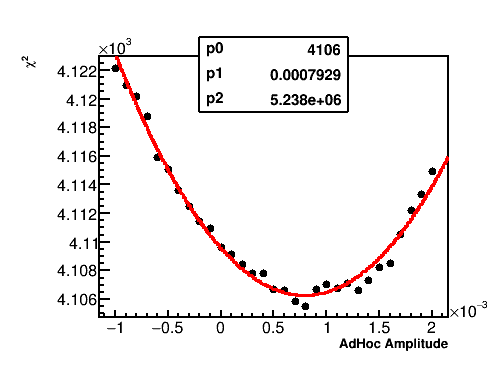
\includegraphics[width=\textwidth]{TMethod_Chi2_Vs_AdHocAmplitude_Canv}
        \caption{T-Method \chisq versus residual gain amplitude. The parabolic fit equation used was $y = p_{2}(x - p_{1})^{2} + p_{0}.$}
    \end{subfigure}% %you need this % here to add spacing between subfigures
    \hspace{1cm}
    \begin{subfigure}[t]{0.45\textwidth}
        \centering
        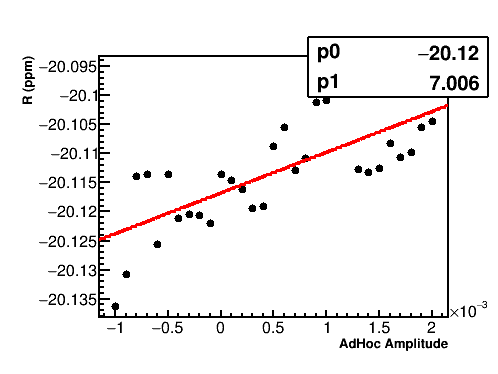
\includegraphics[width=\textwidth]{TMethod_R_Vs_AdHocAmplitude_Canv}
        \caption{T-Method $R$ versus residual gain amplitude. The parameter $p_{1}$ gives the sensitivity of $R$ to the value of the residual gain amplitude, with units in ppm.}
    \end{subfigure}

    \begin{subfigure}[t]{0.45\textwidth}
        \centering
        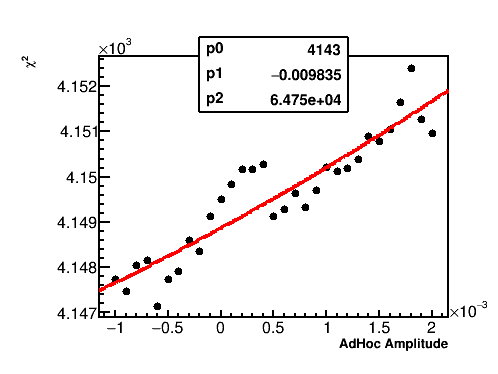
\includegraphics[width=\textwidth]{FullRatio_Chi2_Vs_AdHocAmplitude_Canv}
        \caption{R-Method \chisq versus residual gain amplitude. The parabolic fit equation used was $y = p_{2}(x - p_{1})^{2} + p_{0}.$}
    \end{subfigure}% %you need this % here to add spacing between subfigures
    \hspace{1cm}
    \begin{subfigure}[t]{0.45\textwidth}
        \centering
        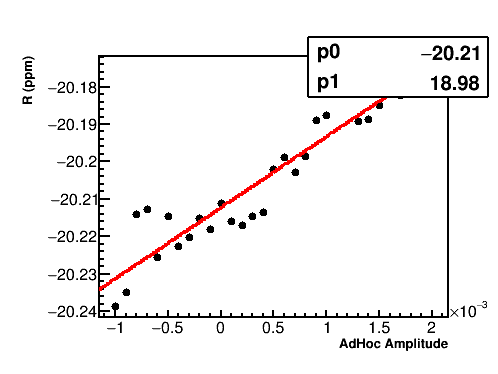
\includegraphics[width=\textwidth]{FullRatio_R_Vs_AdHocAmplitude_Canv}
        \caption{R-Method $R$ versus pileup multiplier. The parameter $p_{1}$ gives the sensitivity of $R$ to the value of the pileup multiplier, with units in ppm.}
    \end{subfigure}
\caption[]{Residual gain amplitude scan. Data are from the 60h dataset.}
\label{fig:AdHocGainScan}
\end{figure}



\begin{landscape}
\begin{figure}[h]
\centering
    \begin{subfigure}[t]{0.4\textwidth}
        \centering
        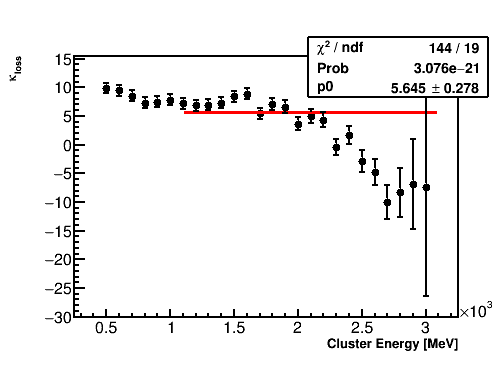
\includegraphics[width=\textwidth]{TMethod_kappa_loss_Vs_EBin_Canv_HK-0}
        \caption{HighKick dataset, $A_{g} = 0$, no residual gain applied.}
    \end{subfigure}% %you need this % here to add spacing between subfigures
    \hspace{1cm}
    \begin{subfigure}[t]{0.4\textwidth}
        \centering
        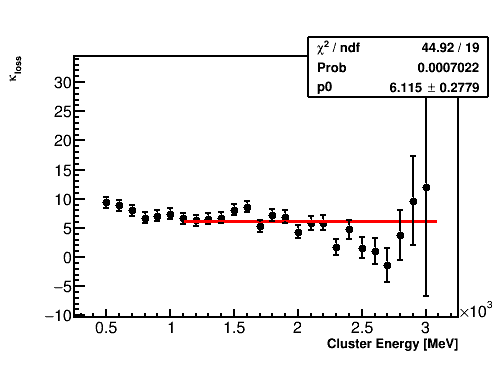
\includegraphics[width=\textwidth]{TMethod_kappa_loss_Vs_EBin_Canv_HK-5p1}
        \caption{HighKick dataset, $A_{g} = 5.1 \times 10^{-4}$, amplitude set to that from the \chisq minima.}
    \end{subfigure}
    \hspace{1cm}
    \begin{subfigure}[t]{0.4\textwidth}
        \centering
        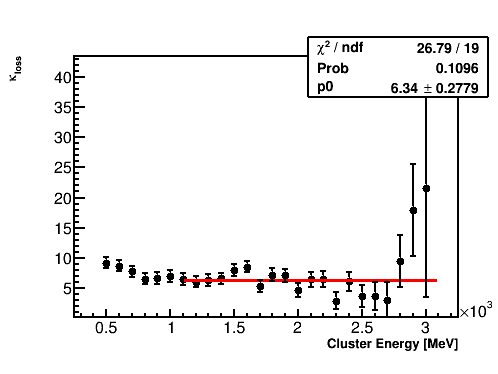
\includegraphics[width=\textwidth]{TMethod_kappa_loss_Vs_EBin_Canv_HK-7p5}
        \caption{HighKick dataset, $A_{g} = 7.5 \times 10^{-4}$, amplitude set to that which flattened out the \K spectrum (approximately).}
    \end{subfigure}

    \begin{subfigure}[t]{0.4\textwidth}
        \centering
        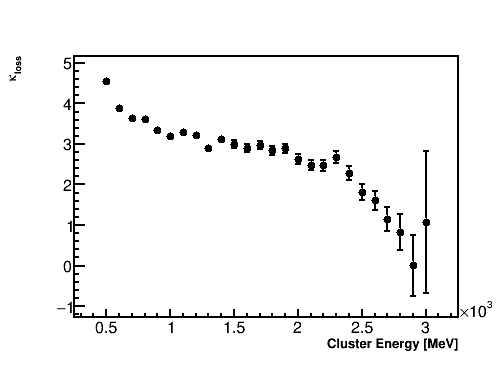
\includegraphics[width=\textwidth]{TMethod_kappa_loss_Vs_EBin_Canv_EG-0}
        \caption{Endgame dataset, $A_{g} = 0$, no residual gain applied.}
    \end{subfigure}% %you need this % here to add spacing between subfigures
    \hspace{1cm}
    \begin{subfigure}[t]{0.4\textwidth}
        \centering
        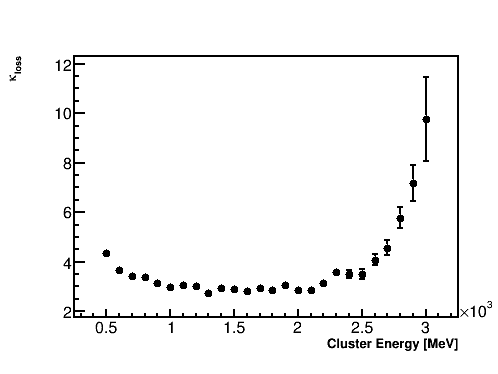
\includegraphics[width=\textwidth]{TMethod_kappa_loss_Vs_EBin_Canv_EG-11p2}
        \caption{Endgame dataset, $A_{g} = 11.2 \times 10^{-4}$, amplitude set to that from the \chisq minima.}
    \end{subfigure}
    \hspace{1cm}
    \begin{subfigure}[t]{0.4\textwidth}
        \centering
        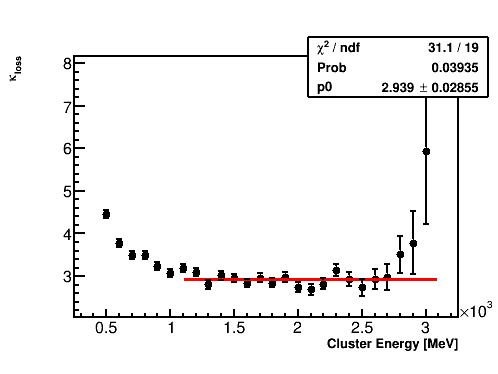
\includegraphics[width=\textwidth]{TMethod_kappa_loss_Vs_EBin_Canv_EG-6p0}
        \caption{Endgame dataset, $A_{g} = 6.0 \times 10^{-4}$, amplitude set to that which flattened out the \K spectrum (approximately).}
    \end{subfigure}
\caption[]{\K versus energy bin, for the HighKick (top) and Endgame (bottom) datasets, with different values for the residual gain amplitude $A_{g}$. \K falls off as a function of energy which is one of the pieces of evidence for the need of a residual gain correction. At low energies \K rises, which is understood to be due to noise hits which increases the lost muon spectra at those energies.}
\label{fig:EBinKloss}
\end{figure}
\end{landscape}



\begin{table}[h]
\centering
% \setlength\tabcolsep{10pt}
\renewcommand{\arraystretch}{1.2}
\begin{tabularx}{0.9\linewidth}{XHGHG}
  \hline
    \multicolumn{5}{c}{\textbf{Residual Gain Tests}} \\
  \hline\hline
            & \multicolumn{2}{c}{$\chi^{2}_{min}$} & \multicolumn{2}{c}{flat $\kappa_{loss}$} \\
  \cmidrule(lr){2-3}\cmidrule(lr){4-5}
    Dataset & \multicolumn{1}{c}{$A_{g} \times 10^{-4}$} & \multicolumn{1}{c}{p value} & \multicolumn{1}{c}{$A_{g} \times 10^{-4}$} & \multicolumn{1}{c}{p value} \\
  \hline
    60h & 8.5 & 0.81 & 8.5 & 0.81 \\
    HighKick & 5.1 & \sim 0 & 7.5 & 0.11 \\
    9d & 8.4 & 0.17 & 10.0 & 0.25 \\
    Endgame & 11.2 & \sim 0 & 6.0 & 0.04 \\
  \hline
\end{tabularx}
\caption[]{Residual gain amplitudes as determined from the \chisq minima or flat \K procedures. P values are given for a straight fit line to the \K versus energy bin spectra from \SIrange{1.1}{3.1}{\GeV} after applying the residual gain correction with those same amplitudes.}
\label{tab:AdHocGainTests}
\end{table}



\tabref{tab:AdHocGainErr} gives the \DR values when applying the residual gain correction. These \DR values with minus without the correction are taken conservatively as the systematic uncertainty due to the potential need for such a residual gain correction. Because the flat \K procedure is more physically motivated, the associated values are taken as the final systematic uncertainties. As shown the systematic uncertainties range up to about 30~ppb depending on the dataset, and is one of the larger systematic uncertainties in the analysis.


As a last note, it should immediately be apparent that the \K energy spectrum was not perfectly flat, even with the residual gain correction applied. Beyond random statistical fluctuations, it rises up at high energy bins, and no $A_{g}$ value was found which could better flatten out the spectrum. This is understood to be an effect of the pileup correction applied, potentially due to the lack of triples included in the correction. With a better pileup algorithm, this effect should go away. Because the systematic uncertainty is taken conservatively as the \DR value with minus without the correction applied, this was deemed acceptable for the Run~1 analysis.




\begin{table}[h]
\centering
% \setlength\tabcolsep{10pt}
\renewcommand{\arraystretch}{1.2}
\begin{tabularx}{0.8\linewidth}{XOOK}
  \hline
    \multicolumn{4}{c}{\textbf{Systematic Uncertainty Due to Residual Gain}} \\
  \hline\hline
    Dataset & \thead{Fit Method} & \multicolumn{1}{c}{$\chi^{2}_{min}$ $\Delta R$} & \multicolumn{1}{c}{flat $\kappa_{loss}$ $\boldsymbol{\Delta R}$}  \\
  \hline
    \multirow{2}{*}{60h} & T & 28.7 & 28.7 \\
                         & R & 22.9 & 22.9 \\
  \hline
    \multirow{2}{*}{HighKick} & T & 1.0 & 11.8 \\
                              & R & 1.8 & 15.3 \\
  \hline
    \multirow{2}{*}{9d} & T & 18.1 & 24.4 \\
                        & R & 15.2 & 19.1 \\
  \hline
    \multirow{2}{*}{Endgame} & T & 29.9 & 18.8 \\
                             & R & 8.5 & 6.7 \\
  \hline
\end{tabularx}
\caption[]{Systematic uncertainties due to residual gain, with an applied amplitude determined from either the minimum of a \chisq scan or that which flattened out the \K versus energy spectra. The latter column is bold since those numbers are those which are taken as the systematic uncertainties. In general both procedures produce the same order of magnitude systematic uncertainties, except for the HighKick where the latter procedure produces larger values. Units are in ppb.}
\label{tab:AdHocGainErr}
\end{table}



